\subsubsection{Sprint goal}
L'obiettivo dello sprint finale è stato quello di implementare il Fantacitorio (richiesto allo sprint precedente), concludere gli scacchi e 
integrare le richieste del cliente emerse dalla sprint review precedente nel prodotto finale.\\
In particolare sono state previste le seguenti funzionalità:
\begin{itemize}
    \item Per il Fantacitorio:
    \begin{itemize}
        \item Visualizzazione e modifica della classifica settimanale
        \item Visualizzazione della classifica generale
        \item Visualizzazione delle squadre degli altri giocatori
        \item Ricerca della squadra di uno specifico utente
        \item Statistiche sulla classifica
    \end{itemize}
    \item Per gli scacchi:
    \begin{itemize}
        \item Pubblicazione della scacchiera come tweet
        \item Raccolta e selezione della mossa dell'avversario a maggioranza
    \end{itemize}
    \item Per i giochi televisivi:
    \begin{itemize}
        \item Visualizzazione dei più vincenti in un periodo di tempo
    \end{itemize}
\end{itemize}


\subsubsection{Backlog}
\userstory%
{Come interessato al Fantacitorio,\\voglio vedere e poter aggiornare una sintesi settimanale dei punteggi dei politici\\per vedere chi sta vincendo.}%
{11\\(4 frontend + 7 backend)}%
{Avere una lista di tutti i politici con i loro relativi punteggi, visualizzarne una sintesi e poter modificarla.}%
{Verificare il corretto parsing dei tweet contenenti i punteggi.}
{Fantacitorio}

\userstory%
{Come interessato al Fantacitorio,\\voglio vedere una classifica cumulativa di punteggi di ogni politico\\per capire chi sta vincendo.}%
{5\\(2 frontend + 3 backend)}%
{Visualizzare una classifica cumulativa con i punti di ogni politico in ordine decrescente.}%
{Verificare che la classifica sia coerente con i punteggi settimanali.}
{Fantacitorio}

\userstory%
{Come interessato al Fantacitorio,\\voglio sfogliare le immagini delle squadre degli altri partecipanti\\per vedere contro chi competo.}%
{7\\(3 frontend + 4 backend)}%
{Visualizzare, in una pagina, tutte le foto delle squadre partecipanti al Fantacitorio.}%
{Verificare manualmente che l'algoritmo sia in grado di riconoscere correttamente le immagini contenenti una squadra.}
{Fantacitorio}

\userstory%
{Come interessato al Fantacitorio,\\voglio poter cercare un utente e vedere se partecipa o meno e mostrare la sua squadra\\per cercare chi gioca.}%
{5\\(2 frontend + 3 backend)}%
{Possibilità di cercare un utente per username e controllare se possiede una squadra, in caso affermativo mostrarla.}%
{Verificare che cercando un utente che partecipa al Fantacitorio, la sua squadra sia visibile.}
{Fantacitorio}

\userstory%
{Come giocatore di scacchi,\\voglio che la scacchiera venga pubblicata\\in modo tale che gli utenti vedano la mossa scelta.}%
{3\\(3 backend)}%
{Pubblicare un tweet con la foto della scacchiera allo stato attuale.}%
{Verificare manualmente che il tweet sia stato pubblicato.}
{Scacchi}

\userstory%
{Come giocatore di scacchi,\\voglio che gli utenti di Twitter scelgano, a maggioranza, la mossa dell'avversario\\per avanzare nella partita.}%
{4\\(1 frontend + 3 backend)}%
{Scelta di una mossa in base alla maggioranza dei voti presenti nei commenti del post pubblicato.}%
{Verificare che la mossa scelta sia quella proposta dal maggior numero di utenti.}
{Scacchi}

\userstory%
{Come spettatore de \#leredita,\\voglio visualizzare colui/colei che ha indovinato più volte nel corso delle puntate,\\per sapere chi è più bravo/a.}%
{5\\(2 frontend + 3 backend)}%
{Possibilità di visualizzare, giorno per giorno, una classifica con le persone con più parole indovinate.}%
{Verificare che gli utenti visualizzati abbiano effettivamente vinto il numero di volte indicato.}
{L'Eredità}

\userstory%
{Come spettatore de \#reazioneacatena,\\voglio visualizzare colui/colei che ha indovinato più volte nel corso delle puntate,\\per sapere chi è più bravo/a.}%
{1\\(1 backend)}%
{Possibilità di visualizzare, giorno per giorno, una classifica con le persone con più parole indovinate.}%
{Verificare che gli utenti visualizzati abbiano effettivamente vinto il numero di volte indicato.}
{Reazione a catena}

\userstory%
{Come interessato al Fantacitorio,\\voglio visualizzare delle statistiche interessanti nella classifica\\per vedere chi sta andando bene e chi no.}%
{3\\(1 frontend + 2 backend)}%
{Mostrare statistiche interessanti nella pagina della classifica, come ad esempio “best climber”, “best average” e “best single score”.}%
{Verificare che le statistiche siano in linea con la classifica.}
{Fantacitorio}


\subsubsection{Esito sprint}
Lo sprint è terminato con la conclusione di tutte le user stories pianificate.\\
\begin{figure}[H]
    \centering
    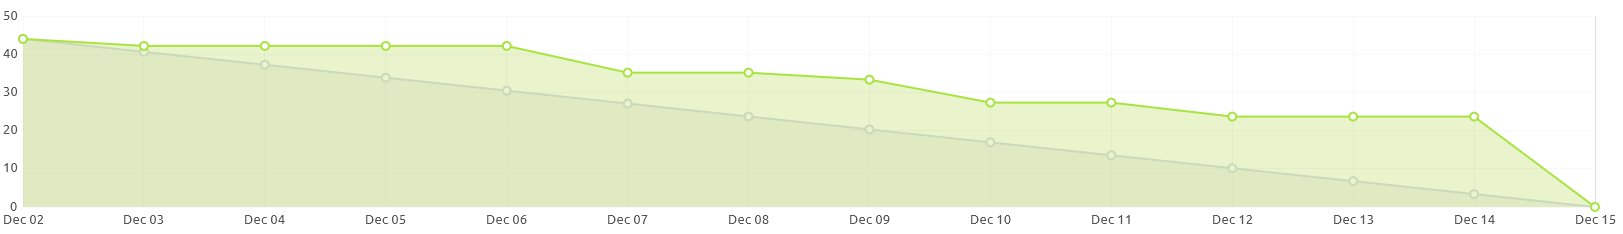
\includegraphics[width=15cm]{./img/sprint4/burndown.png}
    \caption{Burndown sprint 4}
\end{figure}
La distribuzione delle ore di lavoro è risultata disomogenea, con un'importante concentrazione all'ultimo giorno dello sprint.
\begin{figure}[H]
    \centering
    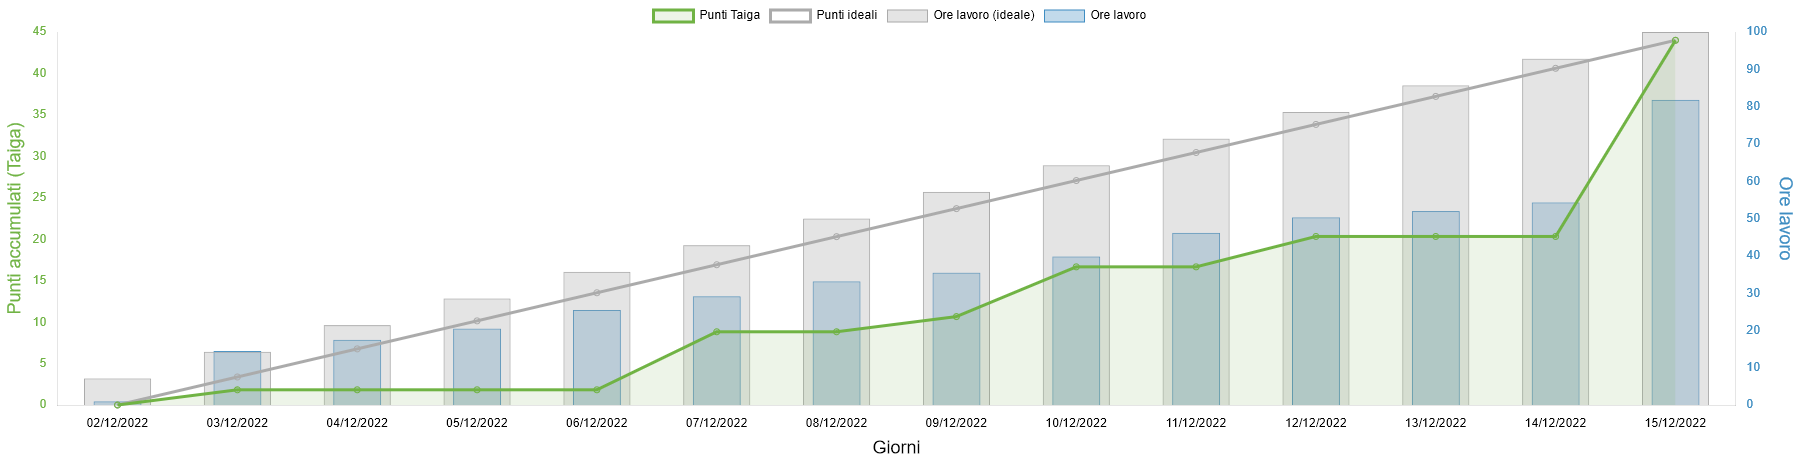
\includegraphics[width=15cm]{./img/sprint4/worktime.png}
    \caption{Progresso dei punti (asse a sinistra) e ore di lavoro (asse a destra)}
\end{figure}


\subsubsection{Retrospettiva}
Alla retrospettiva il team ha evidenziato i seguenti aspetti positivi:
\begin{itemize}
    \item Una buona reazione alle modifiche del backlog
    \item Un incremento significativo nei test (del frontend)
\end{itemize}
È stato invece evidenziato come aspetto negativo un mal bilanciamento del lavoro, concentrato tutto alla fine dello sprint.
\begin{figure}[H]
    \centering
    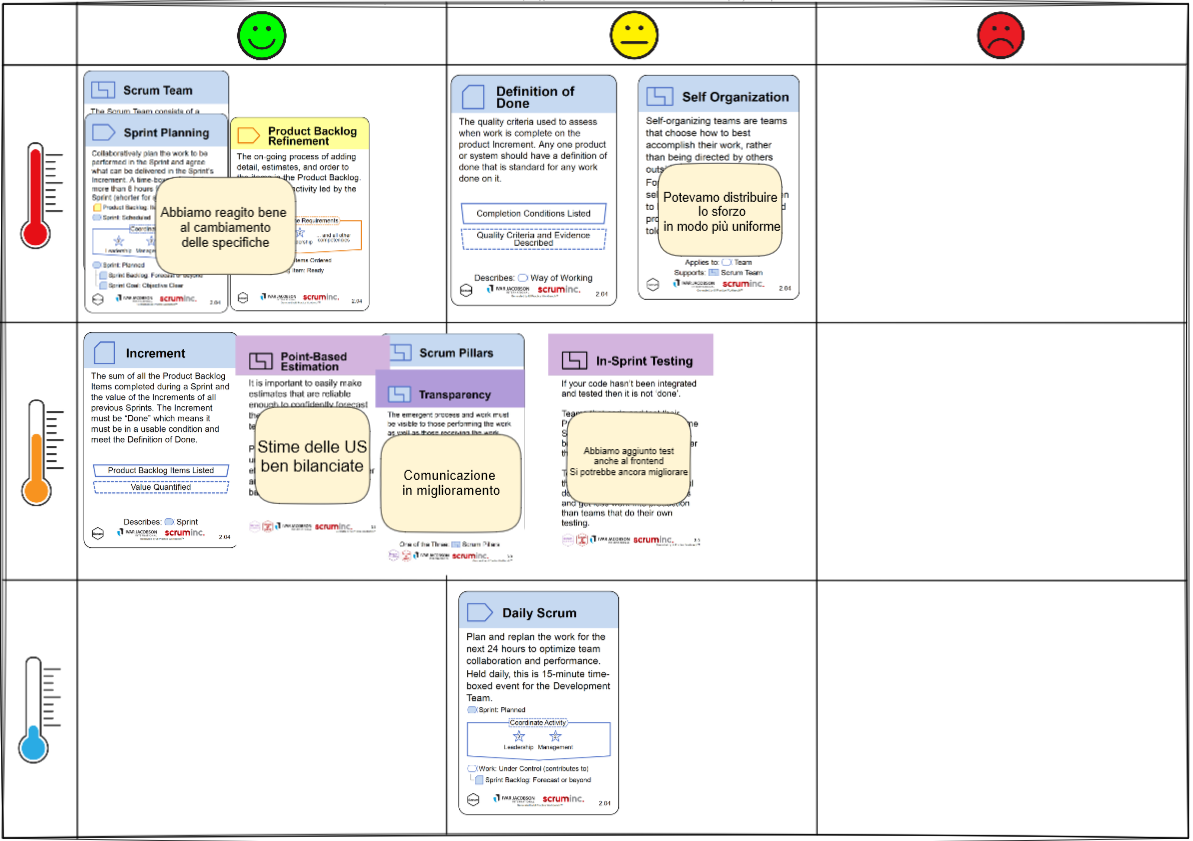
\includegraphics[width=15cm]{./img/sprint4/retrospettiva.png}
    \caption{Retrospettiva del 18/12/2022}
\end{figure}

\subsubsection{Qualità del codice}
I risultati delle analisi effettuate da Sonarqube sul codice sorgente sono i seguenti:
\begin{figure}[H]
    \centering
    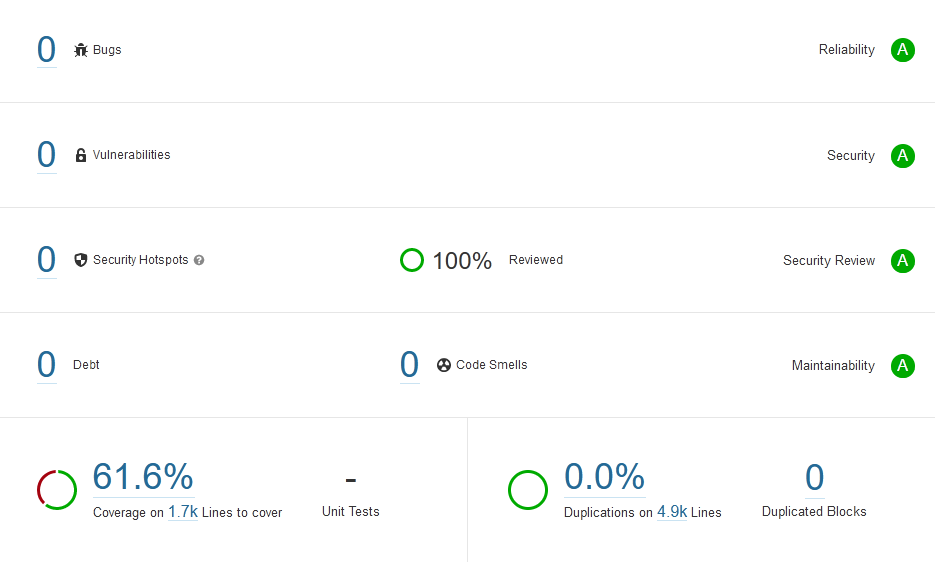
\includegraphics[width=\linewidth]{./img/sprint4/sonarqube.png}
    \caption{Risultato dell'analisi di Sonarqube}
\end{figure}
Tutte le segnalazioni sono state risolte e il coverage dei test sul codice finale è del 61,6\%.\\
Più nel dettaglio la copertura dei test sulle varie sezioni di codice (suddivisione basata sull'organizzazione del file system) è la seguente:
\begin{center}
    \begin{tabular}{|c|c|}
        \hline
        \textbf{Sezione} & \textbf{\% di coverage (righe totali)} \\
        \hline
        \texttt{modules} & 79,9\% (1136) \\
        \hline
        \texttt{controllers} & 66,9\% (207) \\
        \hline
        \texttt{middlewares} & 94\% (122) \\
        \hline
        \texttt{routes} & 100\% (34) \\
        \hline
        \texttt{models} & 100\% (279) \\
        \hline
        \texttt{sockets} & 61,8\% (322) \\
        \hline
        \hline
        \texttt{frontend} & 26,9\% (2524) \\
        \hline
    \end{tabular}
\end{center}